\documentclass{beamer}

\mode<presentation>
{
  \usetheme{Warsaw}
  \useoutertheme{infolines}
  \usecolortheme[RGB={28,13,151}]{structure}
  %\usetheme[height=7mm]{Rochester}
  % or ...

  \setbeamercovered{transparent}
  % or whatever (possibly just delete it)
}

\usepackage{multicol}
\usepackage{verbatim} 
\usepackage{listings}
\usepackage{tikz}
\usepackage{tikzsymbols}
\usetikzlibrary{arrows}
\usetikzlibrary{shapes}
\tikzstyle{block}=[draw opacity=0.7,line width=1.4cm]

\lstloadlanguages{C++}
\lstnewenvironment{code}
	{%\lstset{	numbers=none, frame=lines, basicstyle=\small\ttfamily, }%
	 \csname lst@SetFirstLabel\endcsname}
	{\csname lst@SaveFirstLabel\endcsname}
\lstset{% general command to set parameter(s)
	language=C++, basicstyle=\footnotesize\ttfamily, keywordstyle=\slshape,
	emph=[1]{tipo,usa}, emphstyle={[1]\sffamily\bfseries},
	morekeywords={tint,forn,forsn},
	basewidth={0.47em,0.40em},
	columns=fixed, fontadjust, resetmargins, xrightmargin=5pt, xleftmargin=15pt,
	flexiblecolumns=false, tabsize=2, breaklines,	breakatwhitespace=false, extendedchars=true,
	numbers=left, numberstyle=\tiny, stepnumber=1, numbersep=9pt,
	frame=l, framesep=3pt,
}

\usepackage[spanish]{babel}
% or whatever

\usepackage[utf8]{inputenc}
% or whatever

\usepackage{times}
\usepackage[T1]{fontenc}
% Or whatever. Note that the encoding and the font should match. If T1
% does not look nice, try deleting the line with the fontenc.


\title{Programación Dinámica}  % (optional, use only with long paper titles)


\author[Agustín Gutiérrez] % (optional, use only with lots of authors)
{~Agustín Santiago Gutiérrez}
% - Give the names in the same order as the appear in the paper.
% - Use the \inst{?} command only if the authors have different
%   affiliation.
\institute[UBA-FCEN] % (optional, but mostly needed)
{
  %\inst{1}
  Facultad de Ciencias Exactas y Naturales\\
  Universidad de Buenos Aires
}
\date % (optional, should be abbreviation of conference name)
{Septiembre 2017}

% Acá se puede insertar el logo de la UBA
% \pgfdeclareimage[height=0.5cm]{university-logo}{university-logo-filename}
% \logo{\pgfuseimage{university-logo}}



% Delete this, if you do not want the table of contents to pop up at
% the beginning of each subsection:
\AtBeginSubsection[]
{
  \begin{frame}{Contenidos}
  \footnotesize
  \begin{multicols}{2} 
    \tableofcontents[currentsection, currentsubsection]
  \end{multicols}
  \end{frame}
}

\DeclareMathOperator*{\mimin}{min}
\DeclareMathOperator*{\mimax}{max}

% If you wish to uncover everything in a step-wise fashion, uncomment
% the following command: 

%\beamerdefaultoverlayspecification{<+->}


\begin{document}
\pgfdeclarelayer{background}
\pgfsetlayers{background,main}
\begin{frame}
  \titlepage
\end{frame}


\begin{frame}{Soluciones recursivas a problemas}

  \begin{itemize}
   \item Muchos algoritmos de utilidad son recursivos: para resolver un problema, se utilizan las soluciones a \textbf{subproblemas} fuertemente relacionados.
   \item En estos algoritmos:
       \begin{itemize}
            \item Se \textbf{divide} el problema en ``varios'' subproblemas
               \begin{itemize}
                    \item 0 (casos base)
                    \item 1 o más (casos recursivos)
               \end{itemize} 
            \item Estos se resuelven utilizando el mismo algoritmo
            \item Se \textbf{utilizan} esas subsoluciones para resolver el problema original
       \end{itemize}
   \item Ejemplo: Divide and Conquer (Algoritmos II)
  \end{itemize}
  
\end{frame}

\begin{frame}{¿En qué consiste programación dinámica?}
  \begin{itemize}
   \item Técnica de solución de problemas \textbf{recursiva} (como D\&C)
   \item Diferencia esencial: 
          \begin{itemize}
              \item Se aplica D\&C cuando los subproblemas que se resuelven \\ \textbf{son independientes entre sí}
              \item Se aplica programación dinámica cuando los subproblemas \\ \textbf{no son independientes entre sí}
          \end{itemize}  
   \item Cuando hay \textbf{superposición de subproblemas}, un algoritmo de Divide and Conquer realizaría \textbf{el mismo} trabajo múltiples veces
   \item Lo anterior ocurre ya que la solución a un mismo subproblema puede
   ser \textbf{recalculada} muchas veces si se la reutiliza como parte de varios subproblemas más grandes.
  \end{itemize}
    
\end{frame}

\begin{frame}{¿En qué consiste programación dinámica? (2)}
  \begin{itemize}
   \item Solución: usar programación dinámica.
   \item PD propone \textbf{almacenar} las soluciones a subproblemas ya calculados
   \item Almacenar las soluciones permite calcularlas \textbf{una sola vez}, y luego leer el valor ya calculado cuando se lo vuelve a necesitar.
   \item PD = D\&C + \textbf{caching}
  \end{itemize}
    
\end{frame}

\begin{frame}{Problemas de optimización}
    \begin{itemize}
        \item Uno de los usos más importantes es en problemas de \textbf{optimización}: Se busca una solución que maximice un cierto puntaje u objetivo, en un espacio de soluciones posibles
        \item Para poder aplicar D\&C o PD (técnicas recursivas) debe cumplirse el \textbf{principio del óptimo}: 
        \begin{itemize}
            \item \textbf{Las partes de una solución óptima} a un problema, deben ser \textbf{soluciones óptimas de los correspondientes subproblemas}
            \item Permite obtener una solución óptima al problema original a partir de soluciones óptimas de los subproblemas
        \end{itemize}
        \item Ejemplo donde \textbf{SI} se cumple: \\ \textit{Ordenar con quicksort}
        \item Ejemplo donde \textbf{NO} se cumple: \\ \textit{Calcular un camino máximo simple entre $u$ y $v$ en un grafo}
    \end{itemize}
\end{frame}

\begin{frame}{El esquema general (según el libro de CLRS)}
    Los algoritmos de programación dinámica se pueden organizar típicamente en 4 pasos que responden al siguiente esquema general:
   \begin{enumerate}
   \item Caracterizar la \textbf{estructura} de una solución (óptima)
   \item Definir \textbf{recursivamente} el valor de una solución (óptima)
   \item Computar el \textbf{valor} de una solución (óptima). Se calcula de manera \textit{bottom-up} (CLRS) o \textit{top-down} (``memoization'')
   \item (A veces) Construir una \textbf{solución} óptima a partir de la información obtenida en el paso 3
  \end{enumerate}
    El paso 4 no siempre es necesario, ya que si solamente nos interesa el valor o puntaje de una solución óptima, pero no la solución en sí, muchas veces podemos evitar este paso.

    Además, en problemas que no son de optimización, generalmente el paso 4 no aplica (Fibonacci, calcular \textbf{cantidad} de soluciones, etc)

\end{frame}

\begin{frame}{Problema ``de las monedas''}

\small

	(Parte principal del ejercicio 3.10, práctica 3):
    
\ 

	Dadas varias monedas, de valores posiblemente distintos, dar un cierto vuelto utilizando la mínima cantidad de ellas posible.
    
\ 
    
    Más formalmente: Dadas $n$ monedas, cuyos valores están dados por $v_1, v_2, \cdots, v_n \in \mathbb{Z}_{>0}$, y un $T \in \mathbb{Z}_{>0}$, se debe dar un $I \subseteq \{1,2,3, \cdots, n \}$ tal que
    $\sum_{i \in I}{v_i} = T$, y $|I|$ sea mínimo.
    
%    \in \mathbb{N}^{m \times n}$ una matriz de números naturales. Se desea obtener un camino que empiece en la casilla superior
%    izquierda $(1,1)$, termine en la casilla inferior derecha $(m,n)$ y tal que minimice la suma de los valores de las casillas por
%    las que pasa. En cada casilla $(i,j)$ hay dos movimientos posibles: ir hacia abajo (a la casilla $(i+1, j)$), o ir hacia la
%    derecha (a la casilla $(i, j+1)$).
%   \begin{itemize}
%   \item[a] Diseñar un algoritmo eficiente basado en programación dinámica que resuelva este problema.
%   \item[b] Determinar la complejidad del algoritmo propuesto (temporal y espacial).
%   \item[c] Exhibir el comportamiento del algoritmo sobre la matriz que aparece a continuación.
%  \end{itemize}
%                \[ \left [  \begin{array}{cccc}
%2 & 8 & 3 & 4 \\
%5 & 3 & 4 & 5 \\
%1 & 2 & 2 & 1 \\
%3 & 4 & 6 & 5 \\
% \end{array} \right ] \]
%
\end{frame}

\begin{frame}{Estructura de una solución}
    \begin{itemize}
        \item Nuestro objetivo es llegar a un planteo recursivo del problema.
        \item Antes de escribir la fórmula de la solución, tenemos que relacionar la estructura que tiene la solución a un problema, con las soluciones a problemas más chicos.
        \item Algunas ideas generales para este paso:
        \begin{itemize}
            \item Cuando hay muchos elementos ``disponibles'' en el problema (ej: monedas), a veces conviene enfocar en uno particular
            \item Es muy común realizar una división en casos, que abarquen todas las opciones posibles (ej: o usamos esa moneda, o no la usamos)
            \item En este paso, muchas veces ayuda hacer dibujos y ejemplos.
        \end{itemize}
    \end{itemize} 
\end{frame}

\begin{frame}{Estructura de una solución (cont)}
    \begin{itemize}
    \item Ejemplo: $T= 58$, $v = \{10, 25, 10, 10, 5, 3, 5, 20 \}$
    \item Hay únicamente dos posibilidades:
            \begin{itemize}
                 \item O bien utilizamos la última moneda (la de 20)
                 \item O bien no la utilizamos
            \end{itemize}
    \item Analizamos cómo será $S$, \textbf{una solución óptima} en cada caso:
    \item Si $n \notin S$...
            \begin{itemize}
                 \item Tendrá que sumar $T=58$ con \textbf{las demás} monedas.
                 \item Es decir, $\sum_{i \in S}{v_i} = 58$ con $S \subseteq \{1, 2, 3, \cdots, n-1 \}$
                 \item De todas las maneras de formar $T=58$ con $\{ v_1, v_2, v_3, \cdots, v_{n-1} \}$, la cantidad mínima de monedas posibles tendrá que ser  $|S|$
                 \item Si no fuera así, habría un $S' \subseteq \{1,2, 3, \cdots, n-1 \}$ con $\sum_{i \in S'}{v_i} = 58$ y $|S'| < |S|$. Pero tal $S'$ no puede existir, pues sería una solución al problema original mejor que $S$.
                 \item Es decir, $S$ \textbf{es solución óptima para el subproblema} de formar $T=58$ con las monedas $\{1,2, 3, \cdots, n-1 \}$
            \end{itemize}
    \item Si $n \in S$...
    \end{itemize} 
\end{frame}

\begin{frame}{Estructura de una solución (cont...)}
    \begin{itemize}
    \item Si $n \in S$...
            \begin{itemize}
                 \item Por ejemplo, $S$ tendría la pinta del dibujo:
                 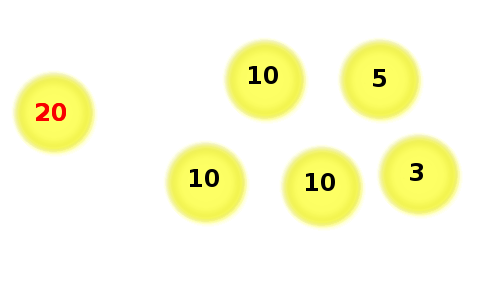
\includegraphics[scale=0.4]{monedas1.png}
                 
                 \item Es decir, $S$ contiene algún subconjunto de monedas, que sabemos que contiene la moneda de valor $v_n = 20$
                 \item ¿Qué podemos decir sobre \textbf{las demás} monedas en $S$?
            \end{itemize}
    
    \end{itemize} 
\end{frame}

\begin{frame}{Estructura de una solución (cont.........)}
    \begin{itemize}
    \item Si $n \in S$...
            \begin{itemize}
                 \item $S = \{n\} \cup S'$, con $\sum_{i \in S'}{v_i} = 38$, $S' \subseteq \{1,2, 3, \cdots, n -1\}$
                 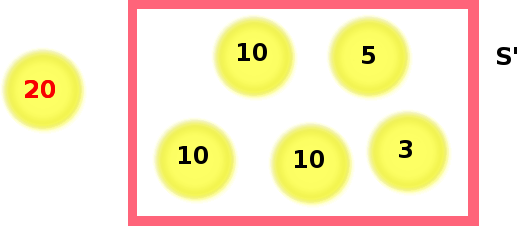
\includegraphics[scale=0.4]{monedas2.png}
                 
                 \item De manera similar a lo que ocurría antes, de todas las maneras de formar $38$ con $\{ v_1, v_2, v_3, \cdots, v_{n-1} \}$, la cantidad mínima de monedas posibles tendrá que ser $|S'|$
                 \item Si no fuera así, habría un $S'' \subseteq \{1,2, 3, \cdots, n -1\}$ con $\sum_{i \in S''}{v_i} = 38$ y $|S''| < |S'|$
                 \item Pero entonces, cambiando $S'$ por $S''$ en nuestra solución... 
            \end{itemize}
    
    \end{itemize} 
\end{frame}

\begin{frame}{Estructura de una solución (cont..................................)}
    \begin{itemize}
    \item Si $n \in S$...
            \begin{itemize}
                 \item ¡Obtendríamos que $\{n\} \cup S''$ es mejor solución que $S$!
                 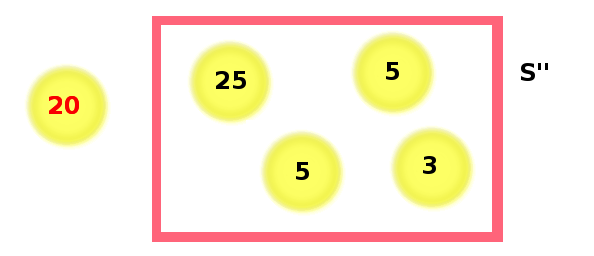
\includegraphics[scale=0.4]{monedas3.png}
                 
                 \item Es decir, $S = \{n\} \cup S'$, donde $S'$ \textbf{es solución óptima para el subproblema} de formar $38$ con las monedas $\{1,2, 3, \cdots, n-1 \}$
            \end{itemize}
    
    \end{itemize} 
\end{frame}

\begin{frame}{Estructura de una solución (resumiendo)}
    \begin{itemize}
        \item Como resultado del análisis anterior, hemos caracterizado una solución óptima $S$ para el problema original:
        \begin{itemize}
            \item Si $n \notin S$, entonces la mejor solución es $S = S_1$, siendo $S_1$ solución óptima para $\{ v_1, v_2, v_3, \cdots, v_{n-1} \}$ dando el mismo vuelto $T$
            \item Si $n \in S$, entonces la mejor solución es $S = \{n\} \cup S_2$, siendo $S_2$ solución óptima para $\{ v_1, v_2, v_3, \cdots, v_{n-1} \}$ dando un vuelto $T - v_n$
        \end{itemize}
        \item Por lo tanto, como esas son las únicas dos posibilidades, $S$ deberá ser la que use menos monedas entre $S_1$ y $\{ n\} \cup S_2$
        \item \textbf{Usando esta caracterización}, podremos elaborar una recursión que calcule la cantidad óptima de monedas necesarias 
    \end{itemize} 
\end{frame}


\begin{frame}{Fórmula recursiva}
\begin{itemize}
    \small
    \item Definimos: $\begin{array}{rcl}f(i, t) & = & \begin{array}{c}\mbox{``mínima cantidad de monedas necesarias} \\ \mbox{para dar un vuelto $t$ con las monedas $\{1, 2, \cdots, i \}$,} \\ \mbox{o $+\infty$ si es imposible''}\end{array}\end{array}$

    \item \textbf{Es muy importante} escribir esta definición de $f$ ``en palabras'': Si no sabemos \textbf{qué} queremos calcular con $f$, es imposible saber si la recursión que estamos dando es correcta o no.
    
    \item Como nuestro objetivo final es resolver el problema, también es importante decir \textbf{cómo se usa} $f$ para obtener la respuesta al problema.
    
    \item En este caso, la cantidad óptima de monedas necesarias para dar el vuelto pedido es simplemente $f(n, T)$:
      \begin{itemize}
         \item Por la definición de $f$, esa es la cantidad mínima necesaria para dar un vuelto $T$ usando las monedas $\{1, 2, \cdots, n \}$
         \item Como esas son \textbf{todas} las monedas disponibles, $f(n,T)$ resulta ser simplemente la mínima cantidad de monedas necesarias, sin restringir cuáles
      \end{itemize}
\end{itemize}    
\end{frame}

\begin{frame}{Fórmula recursiva (cont)}

    $$\begin{array}{rcl} f(i,t) & = & \left \{ \begin{array}{cl} 0 & \mbox{si } i = 0, t = 0 \\ +\infty & \mbox{si } i = 0, t \neq 0 \\ \underbrace{f(i-1,t)}_{S_1} & \mbox{si } i > 0, v_i > t \\ min \left (\underbrace{f(i-1,t)}_{S_1}, \underbrace{1 + f(i-1, t- v_i)}_{\{i\} \cup S_2} \right ) & \mbox{si } i > 0, v_i \leq t \end{array} \right . \end{array} $$ 
\begin{itemize}
    \item Al escribir la fórmula, hemos agregado al análisis anterior:
        \begin{itemize}
            \item Los casos base (correspondientes a $i=0$: no hay monedas)
            \item El caso en el que $v_i > t$, y por lo tanto no es necesario considerar la opción de utilizar la moneda $i$, pues es imposible usarla para pagar el vuelto $t$ 
        \end{itemize}
\end{itemize}    
\end{frame}

\begin{frame}[fragile]{Algoritmo top-down}
\begin{lstlisting}
// d: Diccionario global de soluciones ya calculadas
monedas(i, t):
    IF (i,t) not in d THEN
        IF i=0 and t=0 THEN
            d[i,t] = 0
        IF i=0 and t!=0 THEN
            d[i,t] = +INF
        IF i>0 and v[i]>t THEN
            d[i,t] = monedas(i-1, t)
        IF i>0 and v[i]<=t THEN
            d[i,t] = min(monedas(i-1,t), 1 + monedas(i-1, t-v[i]))
    return d[i,t]
\end{lstlisting}

El diccionario \texttt{d} podría ser una simple matriz (con un valor especial como -1 para indicar un elemento no calculado), por lo que tiene acceso $O(1)$.

Notar que gracias a que guardamos las respuestas, \textbf{nunca se calcula un mismo subproblema más de una vez.}
\end{frame}

\begin{frame}[fragile]{Algoritmo bottom-up}
\begin{lstlisting}
monedas(v, n, T): // v indexado desde 1
    f <- matrizDeEnteros[0..n , 0..T]
    f[0,0] = 0
    FOR t <- 1 TO T DO
        f[0, t] = +INF
    FOR i <- 1 TO n DO
        FOR t <- 0 TO T DO
            IF v[i] > t THEN
                f[i,t] = f[i-1, t]  
            ELSE
                f[i,t] = min(f[i-1,t], 1 + f[i-1, t - v[i])
    RETURN f[n, T]
\end{lstlisting}

La complejidad del algoritmo resultante es $O(nT)$, tanto espacial como temporal. Se puede bajar la complejidad espacial a $O(T)$ (guardando sólo dos filas de la matriz $f$: cada una depende sólo de la anterior)

¿Cuál es la complejidad de la versión top-down?
\end{frame}

\begin{frame}{Comparación general}
\small
$$\begin{array}{c|c}
\mbox{Top-Down (memoization)} & \mbox{Bottom-Up}\\
\hline \\
\mbox{\Smiley Fácil de programar} & \begin{array}{c}\mbox{\Sadey Más difícil: hay que pensar el} \\ \mbox{orden de llenado de la tabla}\end{array}\\
\hline \\
\begin{array}{c}\mbox{\Smiley \Smiley \textbf{Calcula exactamente los}} \\ \mbox{\textbf{subproblemas necesarios}}\end{array} & \mbox{\Sadey Calcula todos los subproblemas}\\
\hline \\
\begin{array}{c}\mbox{\Sadey No permite ahorrar memoria} \\ \mbox{olvidando soluciones}\end{array} & \mbox{\textbf{\Smiley \Smiley Suele permitir ahorrar memoria}}\\
\hline \\
\begin{array}{c} \mbox{(usualmente)} \\ \mbox{\Sadey Mucho peor factor constante} \end{array} & \begin{array}{c} \mbox{(usualmente)} \\ \mbox{\Smiley Mucho mejor factor constante}\end{array}\\
\end{array}$$
\end{frame}


\begin{frame}{Obtener la solución $S$}

\begin{itemize}
    \item Lo anterior es suficiente si solamente necesitamos calcular la cantidad mínima de monedas necesarias.
    \item ¿Pero cómo obtenemos la solución $S$ eficientemente?
    \item Para cada subproblema $f(i, t)$, la solución óptima usa la moneda $i$ o no la usa, según con cuál de las dos opciones se alcance el mínimo.
    \item Podemos almacenar junto a cada valor $f(i, t)$, un booleano que indique con cuál de las dos opciones se obtuvo el mínimo (o bien deducirlo a partir de los valores $f(i,t)$ almacenados)
    \item En este caso, ya no podemos usar la misma técnica para bajar la complejidad espacial del problema, pues necesitamos mantener la matriz en memoria para poder obtener la solución
\end{itemize}

\end{frame}

\begin{frame}{Obtener la solución $S$: ejemplo}

\begin{itemize}
    \item $T= 58$, $n=8$, $v = \{10, 25, 10, 10, 5, 3, 5, 20 \}$
    \item $f(8, 58) = 1 + f(7,38)$, así que usamos la moneda $v_8 = 20$
    \item $f(7, 38) = f(6,38)$
    \item $f(6, 38) = 1 + f(5,35)$, así que usamos la moneda $v_6 = 3$
    \item $f(5, 35) = f(4,35) = f(3, 35)$
    \item $f(3, 35) = 1 + f(2, 25)$, así que usamos la moneda $v_3 = 10$
    \item $f(2, 25) = 1 + f(1, 0)$, así que usamos la moneda $v_2 = 25$
    \item $f(1, 0) = f(0, 0) = 0$
    \item De todo lo anterior, resultó $S=\{2, 3, 6, 8 \}$
    
\end{itemize}

\end{frame}


\begin{frame}{Referencias}
   \begin{itemize}
   \item Introduction to Algorithms, 2nd Edition. MIT Press. Thomas H. Cormen, Charles E. Leiserson, Ronald L. Rivest, Clifford Stein
   Página 323: 15 Dynamic Programming
  \end{itemize}
\end{frame}


\end{document}
